% Copyright 2004 by Till Tantau <tantau@users.sourceforge.net>.
%
% In principle, this file can be redistributed and/or modified under
% the terms of the GNU Public License, version 2.
%
% However, this file is supposed to be a template to be modified
% for your own needs. For this reason, if you use this file as a
% template and not specifically distribute it as part of a another
% package/program, I grant the extra permission to freely copy and
% modify this file as you see fit and even to delete this copyright
% notice.

\documentclass{beamer}
% Replace the \documentclass declaration above
% with the following two lines to typeset your
% lecture notes as a handout:
%\documentclass{article}
%\usepackage{beamerarticle}

% There are many different themes available for Beamer. A comprehensive
% list with examples is given here:
% http://deic.uab.es/~iblanes/beamer_gallery/index_by_theme.html
% You can uncomment the themes below if you would like to use a different
% one:
%\usetheme{AnnArbor}
%\usetheme{Antibes}
%\usetheme{Bergen}
%\usetheme{Berkeley}
%\usetheme{Berlin}
%\usetheme{Boadilla}
%\usetheme{boxes}
%\usetheme{CambridgeUS}
%\usetheme{Copenhagen}
%\usetheme{Darmstadt}
%\usetheme{default}
%\usetheme{Frankfurt}
\usetheme{Goettingen}
%\usetheme{Hannover}
%\usetheme{Ilmenau}
%\usetheme{JuanLesPins}
%\usetheme{Luebeck}
%\usetheme{Madrid}
%\usetheme{Malmoe}
%\usetheme{Marburg}
%\usetheme{Montpellier}
%\usetheme{PaloAlto}
%\usetheme{Pittsburgh}
%\usetheme{Rochester}
%\usetheme{Singapore}
%\usetheme{Szeged}
%\usetheme{Warsaw}

\title{Instalación y optimización de un servidor web}

% A subtitle is optional and this may be deleted
\subtitle{Ingeniería de Servidores}

%\author{Alejandro Alcalde Barros}
% - Give the names in the same order as the appear in the paper.
% - Use the \inst{?} command only if the authors have different
%   affiliation.

\institute[Escuela Técnica Superior Ing. Informática Y Telecomunicaciones] % (optional, but mostly needed)
{
  Universidad de Granada
}
% - Use the \inst command only if there are several affiliations.
% - Keep it simple, no one is interested in your street address.

\date{\today}
% - Either use conference name or its abbreviation.
% - Not really informative to the audience, more for people (including
%   yourself) who are reading the slides online

\subject{Theoretical Computer Science}
% This is only inserted into the PDF information catalog. Can be left
% out.

% If you have a file called "university-logo-filename.xxx", where xxx
% is a graphic format that can be processed by latex or pdflatex,
% resp., then you can add a logo as follows:

% \pgfdeclareimage[height=0.5cm]{university-logo}{university-logo-filename}
% \logo{\pgfuseimage{university-logo}}

% Delete this, if you do not want the table of contents to pop up at
% the beginning of each subsection:
\AtBeginSubsection[]
{
  \begin{frame}<beamer>{Tabla de contenidos}
    \tableofcontents[currentsection,currentsubsection]
  \end{frame}
}

    \usepackage{fontspec} % Allows font customization
    \defaultfontfeatures{Mapping=tex-text,Scale=MatchLowercase}
    \setmainfont{Courier} % Main document font
%    \setmonofont{DroidSansMono}


\usepackage{minted}
\usepackage{mathtools}
\usepackage{amsmath}
\definecolor{fondo}{RGB}{221,221,242}


% Let's get started
\begin{document}

\begin{frame}
  \titlepage
\end{frame}

\begin{frame}{Tabla de contenidos}
  \tableofcontents
  % You might wish to add the option [pausesections]
\end{frame}

% Section and subsections will appear in the presentation overview
% and table of contents.
\section{Compilar e instalar nginx}

\subsection{Preparando el entorno}

\begin{frame}{Instalar dependiencias y descargar nginx}{}
  \begin{itemize}
  \item {
       \mint[bgcolor=fondo,fontsize=\scriptsize]{bash}/apt-get install build-essential libssl-dev libpcre3-dev/
       \pause
  }
  \item {
    Descargar nginx y compilarlo, realizando algunas modificaciones al código
    para modificar la cabecera \emph{Server:} que se mostrará en la respuesta HTTP.
    \mint[bgcolor=fondo,fontsize=\scriptsize]{bash}!wget http://nginx.org/download/nginx-1.4.4.tar.gz!
  }
  \item<3-> {
    Módulos a compilar:
    --with-http\_gzip\_static\_module --sbin-path=/usr/local/sbin
    -with-http\_ssl\_module --without-mail\_pop3\_module --without-mail\_imap\_module
    --without-mail\_smtp\_module --with-http\_stub\_status\_module --with-http\_realip\_module
  }
  \end{itemize}
\end{frame}

\subsection{Configurar y compilar}

% You can reveal the parts of a slide one at a time
% with the \pause command:
\begin{frame}{Configurar y compilar}
  \begin{itemize}
  \item {
    Una vez ejecutado \emph{./configure} con los las opciones anteriores
    \mint[bgcolor=fondo,fontsize=\scriptsize]{bash}/make && make install/
    \pause % The slide will pause after showing the first item
  }
  \item {
    Lo iniciamos
    \mint[bgcolor=fondo,fontsize=\scriptsize]{bash}!nginx!
  }
  % You can also specify when the content should appear
  % by using <n->:
  \item<3-> {
    Nos dirigimos a la direción 127.0.0.1 para comprobar que funciona
        \begin{figure}[H]
        \centering
        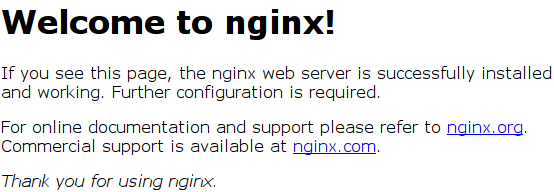
\includegraphics[scale=.2]{./img/instalacionNginx.png}
        \caption{Nginx recién instalado}
        \label{nginx1}
        \end{figure}
  }
  %\item<4-> {
  %  Fourth item.
  %}%
  % or you can use the \uncover command to reveal general
  % content (not just \items):
  %\item<5-> {
  %  Fifth item. \uncover<6->{Extra text in the fifth item.}
  %}
  \end{itemize}
\end{frame}

\section{Instalar PHP-FPM}

\subsection{Añadir repositorios}

\begin{frame}{Pasos necesarios}
  \begin{itemize}
  \item {
        En el \emph{source.list} es necesario añadir el siguiente repositorio
       \mint[bgcolor=fondo,fontsize=\scriptsize]{bash}!deb http://packages.dotdeb.org stable all!
       \pause
  }
  \item<2-> {
    Actualizamos los repositorios y descargamos la llave pública
    \mint[bgcolor=fondo,fontsize=\scriptsize]{bash}!apt-get update!
    \mint[bgcolor=fondo,fontsize=\scriptsize]{bash}!wget http://www.dotdeb.org/dotdeb.gpg!
    \mint[bgcolor=fondo,fontsize=\scriptsize]{bash}!cat dotdeb.gpg | sudo apt-key add -!
    \mint[bgcolor=fondo,fontsize=\scriptsize]{bash}!apt-get install php5-cli php5-suhosin php5-fpm php5-cgi!
    \mint[bgcolor=fondo,fontsize=\scriptsize]{bash}!service php5-fpm start!
  }
  \item<3-> {
    Tras esto hay que realizar unos pequeños cambios en la configuración de nginx para que sepa en qué
    puerto escuchar para procesar los archivos PHP.
  }
  \end{itemize}
\end{frame}

\section{Calcular el número de procesos necesarios}

\subsection{Calcular max\_children}

\begin{frame}{Calcular max\_children}
  \begin{itemize}
  \item {
        Hay tres formas de calcular el número máximo de procesos para php (se modifica en el archívo \emph{/etc/php5/fpm/pools.d}).
        Uno de ellos es
        \begin{theorem}
            $pm.max\_children = (RAM_{total} - RAM_{resto Proc})/ RAM_{mediaPHP}$
        \end{theorem}
       \pause
  }
  \item<2-> {
        El parámetro \emph{start\_servers} se puede calcular en base a:
        \begin{theorem}
            $start\_servers = min\_spare\_servers + (max\_spare\_servers - min\_spare\_servers) / 2$
        \end{theorem}
  }
  \item<3-> {
    El resto de parámetros se calculan conforme se considere que se obtiene el mejor rendimiento.
  }
  \end{itemize}
\end{frame}

% Placing a * after \section means it will not show in the
% outline or table of contents.
\section*{Resumen}

\begin{frame}{Resumen}
  \begin{itemize}
  \item
    Qué no se ha visto en esta presentación
    \begin{itemize}
    \item
      Instalación y configuración de Pagespeed
    \end{itemize}
  \end{itemize}
\end{frame}



% All of the following is optional and typically not needed.
\appendix
\section<presentation>*{\appendixname}
\subsection<presentation>*{Referencias}

\begin{frame}[allowframebreaks]
  \frametitle<presentation>{Referencias}

  \begin{thebibliography}{10}

  \beamertemplatearticlebibitems
  % Start with overview books.

  \bibitem{Author1990}
    Alejandro. %Alcalde.
    \newblock {\em Cómo instalar y configurar Nginx con php5-fpm}.
    \newblock http://elbauldelprogramador.com/how-to/como-instalar-nginx-con-php5-fpm/
  \bibitem{Author19901}
    Guillaume Moigneu.
    \newblock {\em Optimize nginx and PHP-FPM (max\_children)}.
    \newblock http://myshell.co.uk/index.php/adjusting-child-processes-for-php-fpm-nginx/


  %\beamertemplatearticlebibitems
  % Followed by interesting articles. Keep the list short.

  %\bibitem{Someone2000}
  %  S.~Someone.
  %  \newblock On this and that.
  %  \newblock {\em Journal of This and That}, 2(1):50--100,
  %  2000.
  \end{thebibliography}
\end{frame}

\end{document}


